%%
%% Meta: TI nSpire Einführung
%%       Ziel: Damit die Grundoperationen damit durchgeführt werden können.
%%             Damit man sich an den Rechner gewöhnt.
%%

%% Philipp G Freimann Juli 2019 für die BBW
%% Phi BBW-Vorlage für Arbeitsblätter (LaTeX)
%% 2019 - 08 - 18

%% %% %% %%
\documentclass[twoside,12pt,a4paper]{article}%%
\usepackage[paper=a4paper,margin=17mm]{geometry}%%


%% Zentralisiert
%%\usepackage{german} %% Macht Probleme mit grafiken
\usepackage{mciteplus}

\usepackage[dvipsnames,table]{xcolor}

\usepackage{pgfplotstable}
\usepackage{tikz}
\usepackage{tkz-euclide} %% Grid

\usepackage{amsthm}
\usepackage{amsfonts} %% Zahlmengen Z, R, ...


%% THEOREMS?
\usepackage{tcolorbox}
\tcbuselibrary{theorems}
\tcbuselibrary{skins}


\usepackage{fancyhdr}
\usepackage{ngerman}
\usepackage[utf8]{inputenc}


%%\usepackage[dvips]{graphicx}

\usepackage{supertabular}
\usepackage{makeidx}  
\usepackage{ifthen} 

\usepackage{multirow}
\usepackage{listings}

%%\usepackage{color,fancyvrb,fancybox}
\usepackage{multicol}
\usepackage{lastpage}
%%\usepackage{listings}
\usepackage{pstricks}

%% bold typewriter font:
\usepackage[T1]{fontenc}
\usepackage{lmodern}

\usepackage{enumitem}
%\usepackage{enumerate}

\usepackage{float}

\usepackage{titlesec}
\usepackage{textcomp}

%% Kuchendiagramme
%%\usepackage{datapie}

%% für Aufgaben Hervorhebung
%%\usepackage[most]{tcolorbox}
%%\usepackage[standard,framed]{ntheorem}
\usepackage{framed}
\usepackage{mdframed}

%%%%%%%%%%%%%%%%%%%%
%%\usepackage[most]{tcolorbox}

\usepackage[tocindentauto]{tocstyle}

%% für accentset wedge:
\usepackage{accents}

%% Würfel
\usepackage{epsdice}

%% Einbinden von GeoGebra Bildchen:
\usetikzlibrary{shapes.geometric}
\usetikzlibrary{arrows}
\newcommand{\degre}{\ensuremath{^\circ}}

%% Hyperlinks
\usepackage{hyperref}

\hypersetup{
    colorlinks=true,
    linkcolor=blue,
    filecolor=magenta,      
    urlcolor=cyan,
    bookmarks=true,
}

%% bugtracker (part of pgfplots) should be loaded AFTER "hyperref"
%% See: https://texblog.net/hyperref/ AND https://tex.stackexchange.com/questions/16268/warning-with-footnotes-namehfootnote-xx-has-been-referenced-but-does-not-exi
\usepackage{pgfplots}
\pgfplotsset{width=10cm,compat=1.9}

%%\usepackage{fourier}  %% eg overarc (Bogenmaß)

%%%%%%%%%%%%%%%%% L A Y O U T  %%%%%%%%%%%%%%%%%%%%%%%%%%%%
%% 2020-12-27 ph. g. freimann @ bbw.ch
%%

\fancyhf{}%%

\pagestyle{fancy}%%

\renewcommand{\sectionmark}[1]{%%
  \markboth{\thesection{} \ #1}{}%%
}%%

\renewcommand{\subsectionmark}[1]{%%
  \markright{\thesubsection \ #1}%%
}%%

%% Achtung: chaptermark nur im BOOK-Style

\renewcommand{\footrulewidth}{0.4pt}

\parskip4pt
\parindent0pt

\topmargin-2.0cm
\textheight24.4cm

\renewcommand{\arraystretch}{1}%%


\newenvironment{bbwFillInTabular}{%%
%% BEGIN PART:
\renewcommand{\arraystretch}{2.1}
\begin{tabular}%%
}%% END PART:
{\end{tabular}
\renewcommand{\arraystretch}{1}%%
}%% END Environment bbwFillInTabular

%%%%%%%%%%%%%%%%%%%%%%%%%%%%%%%%%%%%%%%%%%%%%%%%%%%%%%%%%%
%%%%%%%%%%%%%%%%%% M A K R O S %%%%%%%%%%%%%%%%%%%%%%%%%%%
%%%%%%%%%%%%%%%%%%%%%%%%%%%%%%%%%%%%%%%%%%%%%%%%%%%%%%%%%%

%%%%%%%%%%%%%%%%%%%%%%%% g e n e r e l l e   M a k r o s %%%%%%%%%%%%%%%%%%%%%%%

%% Info vorab bei \newcommand
%% \newcommand{ - Kommandos können in den Parametern auch Leerzeilen
%%     enthalten
%% \newcommand*{ - Kommandos, also mit *, können jedoch in den
%%    Argumenten KEINE \par (sprich Leerzeilen} enthalten

%% 2019-07-26
%% phi@freimann.eu
%% Makros for BBW-Tex Documents
\usepackage{inputs/bbwColors}

%%%%%%%%%%%%%%%%%% I N C L U D E S   &   I N D E X  %%%%%
\graphicspath{{../img/}}
\graphicspath{{./img/}}

\newcommand*\bbwGraphicRaise[3]{\raisebox{#1}{\includegraphics[width=#2]{#3}}}%%
\newcommand*\bbwGraphic[2]{\bbwGraphicRaise{-5mm}{#1}{#2}}%%
\newcommand*\bbwCenterGraphicRaise[3]{\begin{center}\bbwGraphicRaise{#1}{#2}{#3}\end{center}}
\newcommand*\bbwCenterGraphic[2]{\bbwCenterGraphicRaise{-5mm}{#1}{#2}}%%


%% All in one Skript
\newif\ifisALLINONE
\isALLINONEfalse

%% Blended Learning
%% Insb. MatheNinja Links. Diese sind jedoch in einem anderen Kurs!
\newif\ifisBLENDED
\isBLENDEDfalse


%%%%%%%%% TRAINER Version vs. Schülerversion %%%%%%%%%%%%%
%% Bem. Kein *-Kommando, da die TRAINER-Blöcke auch leerzeilne (\par)
%% enthaltne können
\newcommand\TRAINER[1]{%%
{%%
\ifisTRAINER{\color{BlueGreen}{#1}}%%
\fi%%
}}%%  

\newcommand\TALS[1]{%
{%%
\ifisTALS{#1}%%
\fi%%
}}%

\newcommand\GESO[1]{%
{%%
\ifisGESO{#1}%%
\fi%%
}}%    

\newcommand\BLENDED[1]{%
{%%
\ifisBLENDED{#1}%%
\fi%%
}}%    

\newcommand{\noTRAINER}[1]{{\ifisTRAINER{}\else{#1}\fi}{}}%%



%%\makeatletter
%% Je nach Umgebung "environment" wird das mmPapier breiter oder
%% schmaler
%% bei itemize sollen 16.4 und bei definiton-Boxen 16.8 mm genommen
%% werden.


\usepackage{inputs/mmPapierbreiteSty}


%% Trainer "no" Dotfill
%% If no Trainer: Dotfill
\newcommand*{\TNDF}[1]{\TRAINER{#1}\noTRAINER{\dotfill{}}}%%

\newcommand*{\leserluft}{\vspace{2mm}}

%% Notiz felder 
%% Anwendung:
%% \noteField{10}  
%%  --> Notizfeld mit 10 Leerzeilen
\newcounter{DFCounter}


%%Häuschenpapier
\newcommand{\mmPapierZwei}[2]{\begin{tikzpicture}
%%  \draw[step=4mm,bbwMMFarbe,ultra thin]
%%  \draw[step=4mm,bbwMMFarbe,thick]
  \draw[step=4mm,bbwMMFarbe,line width=0.02mm]
  (0, 0) grid ({#2}, {#1});
\end{tikzpicture}}%%


%% millimeterPapier füllen bis Ende Seite
\newcommand{\mmPapierBisEndeSeite}{

\begin{tikzpicture}

\newdimen\spaceleftOnPage
\spaceleftOnPage=\dimexpr\textheight-\pagetotal-14pt\relax

\pgfmathsetmacro{\gridWidth}{\textwidth        - mod(\textwidth,      4mm)      }
\pgfmathsetmacro{\gridHeight}{\spaceleftOnPage - mod(\spaceleftOnPage,4mm) - 4mm}

\draw [step=4mm,bbwMMFarbe,line width=0.02mm] (0,0) grid (\gridWidth pt,\gridHeight pt);
\end{tikzpicture}%%
\newpage%%
}%% END Makro mmPapieBisEndeSeite


%% Standardbreite für Arbeitsblätter und das Theorieheft
%% Wird in bbwPruefung.sty überschrieben, da dort schmaler
\def\defaultTextBreite{17.6}
\def\unitCMWhatElse{cm}%% wird als Breitenangabe für den nächsten command verwendet

%% Verwendung: \bbwCenterGraphic{\defaultTextBreite}{«img url»}
\def\defaultTextBreiteCM{\defaultTextBreite\unitCMWhatElse}
\newcommand{\mmPapier}[1]{\mmPapierZwei{#1}{\defaultTextBreite}}


%% Notizen Berechungen auf Prüfungsblättern
\newcommand{\platzFuerBerechnungen}[1]{\noTRAINER{

Notizen / Berechnungen:

\mmPapier{#1}}}%% end platzFuerBerechnungen

\newcommand{\platzFuerBerechnungenBisEndeSeite}[1]{\noTRAINER{

Notizen / Berechnungen:

\mmPapierBisEndeSeite}}%% end platzFuerBerechnungen



\newcommand{\platzFuerBerechnungenOhneText}[1]{\noTRAINER{

\mmPapier{#1}}}

%% Die Abkürzung z.\,B. von «Zum Beispiel» hat einen verkleinerten Abstand.
\newcommand*\zB{%
z.\,B.
}

%%
%% Auf der Titelseite steht entweder GESO oder TALS.
%% Dies wird gleich mit der Fußnote angegeben.
%% Dieses Kommando sollte im Kommando «\untertitel» eingesetzt werden.
%%
\newcommand*\ausrichtungAufTitelseite{%
\ifisTALS{TALS\noTRAINER{\footnote{TALS «Technik, Architektur und Life Sciences
(Laboranten)»: Ausrichtung technisches Profil}}}%%
\fi%%
\ifisGESO{GESO\noTRAINER{\footnote{GESO: Ausrichtung \textbf{Ge}sundheit und \textbf{So}ziales}}}%%
\fi}%%

%%%%%%%%%%%%%%%%%%%%%% B B W - M a t h e   F a r b c o d e s  %%%%%%%%%%%%%%%%%%%%%%%%%%%%%%555

\newcommand{\rezeptFarbe}{rezeptFarbe}
\newcommand{\definitionFarbe}{definitionFarbe}
\newcommand{\gesetzFarbe}{gesetzFarbe}
\newcommand{\beispielFarbe}{beispielFarbe}
\newcommand{\bemerkungFarbe}{bemerkungFarbe}

%% Falls gewünscht übersteuren
%  \definecolor{xyz}{HTML}{eeff66}
%  \renewcommand{\beispielFarbe}{xyz}
%

%% Theorem-Styles
\newcommand\theoremlayoutdefinition[4]{\newtcbtheorem[number within=section]{#1}{#2}%
   {theorem style=plain,enhanced,colframe=#3!20!white,colback=#3!20!white,
     coltitle=#3!60!black,fonttitle=\upshape\bfseries,
     %%fontupper=\itshape,
    %%drop fuzzy shadow=blue!50!black!50!white,
    terminator sign={:},
    borderline north={0.5mm}{0pt}{#3}, borderline south={0.5mm}{0pt}{#3}
}{#4}}



%% Farben für rezept, definition und gesetz von Marthale übernommen.
%% Verwendung mit * unterbindet die Nummerierung \begin{gesetz*}{Blah}{xy} ...\end {gesetz*}
\theoremlayoutdefinition{rezept}{Rezept}{\rezeptFarbe}{R}
\theoremlayoutdefinition{definition}{Definition}{\definitionFarbe}{D}
\theoremlayoutdefinition{gesetz}{Gesetz}{\gesetzFarbe}{G}%% was green
\theoremlayoutdefinition{beispiel}{Beispiel}{\beispielFarbe}{B}
\theoremlayoutdefinition{bemerkung}{Bemerkung}{\bemerkungFarbe}{M}

%%
%% Force a blank page, when \newpage does not work
%%
\def\blankpage{%
	\clearpage%
	\null%
	\clearpage}%%

\newcommand{\Lueckentext}[1]{\,\,\noTRAINER{\dotfill}\TRAINER{#1}}


\newcommand{\LoesungsRaumCM}[2]{\,\,\noTRAINER{\underline{\hspace{#1}}}\TRAINER{#2}}

\newcommand{\LoesungsRaum}[1]{\LoesungsRaumCM{30mm}{#1}}
\newcommand{\LoesungsRaumKurz}[1]{\LoesungsRaumCM{15mm}{#1}}
\newcommand{\LoesungsRaumLang}[1]{\LoesungsRaumCM{45mm}{#1}}


%% TI nSpire
\def\tinspire{\texttt{TI-nSpire}}

%% TI 30 Pro Mathprint Button Images
\def\tiprobuttonbreite{10mm}
\def\nspirebuttonbreite{8.6mm}

%%\def\sec{\raisebox{-2mm}{\includegraphics[width=\buttonbreite{}]{img/tiprobuttonimages/2nd.png}}}
\newcommand{\tiprobutton}[1]{\raisebox{-2mm}{\mbox{\,\includegraphics[width=\tiprobuttonbreite{}]{img/tiprobuttonimages/#1.png}\,}}}

\newcommand{\nspirebutton}[1]{\raisebox{-2mm}{\mbox{\,\includegraphics[width=\nspirebuttonbreite{}]{img/nspirebuttonimages/#1.png}\,}}}

%% Counter  für Aufgaben
%% Bei jedem Part wird die Aufgabennummer zurückgesetz auf 1
\newcommand{\bbwPartID}{AA1}
\newcommand{\bbwAufgabenBlockID}{}
\newcounter{bbwAufgabenNummerCounter}[part]
\setcounter{bbwAufgabenNummerCounter}{1}
\newcommand{\bbwAufgabenNummer}{\arabic{bbwAufgabenNummerCounter}}
\newcommand{\nextBbwAufgabenNummer}{\stepcounter{bbwAufgabenNummerCounter}}
\newcommand{\aufgSubLabel}{{\color{blue}\bbwAufgabenNummer. \alph*)}}

%% Benutze außerhalb der bbwAufgabenblöcke folgendes Kommando, um an die
%% nächste Aufgabennummer zu kommen. Dies z. B. wenn ein längerer Text vor der Aufgabe steht,
%% der auch schon diese Bezeichnung erhalten sollte
\newcommand{\bbwActAufgabenNr}{{\color{blue}\bbwAufgabenNummer. {\small[\bbwAufgabenBlockID]}}}


\newenvironment{bbwAufgabenBlock}{%% Begin environment Part:

\bbwActAufgabenNr{}
%%{\color{blue}\bbwAufgabenNummer. {\small[\bbwAufgabenBlockID]}}
\begin{enumerate}[label=\aufgSubLabel]
}%% Ende der Präambel
{%% END Part:
\end{enumerate}
\nextBbwAufgabenNummer
}%% END environment bbwAufgabenBlock

%%%%%%%%%%%%%%%%%%%%%%%%%%%%

%% Weblinks und Mathe Ninja Links

\newcommand{\weblink}[2]{\href{#2}{#1}}

\newcommand{\olatBBWLogo}{
\includegraphics[width=15mm]{logos/traube.pdf}}%%
\newcommand{\externerLinkEPS}{
\includegraphics[width=15mm]{logos/extLink.pdf}}%%
\newcommand{\youtubeLogo}{\includegraphics[width=15mm]{logos/youtube.png}}%%


%%
%% #1: Text
%% #2: URL
%% #3: Aufgabennummern
%% #4: optional weitere Logos oder leer lassen {}
\newcommand{\externalLink}[4]{%%
\begin{tabular}{|lp{111mm}|}\hline%%
\multicolumn{2}{|p{172mm}|}{\cellcolor{aufgabenFarbe}#3}\\
\weblink{\raisebox{-5mm}{\externerLinkEPS{}}}{#2} {#4}  & \weblink{#1}{#2}\\\hline
\multicolumn{2}{|p{172mm}|}{\weblink{#2}{#2}}\\\hline
\end{tabular}%%
\vspace{1mm}
}%% END Command externalLink

%% #1: URL
%% #2: Text
\newcommand{\youtubeLink}[2]{%%
\externalLink{#2}{#1}{Youtube}{\raisebox{-5mm}{\youtubeLogo{}}}
}%%

%%
%% #1: Typ-Logo (eg. LOGO auf MatheNinja)
%% #2: Typ-Name (eg «Mathe Ninja»
%% #3: URL
%% #4: Aufgaben Name
\newcommand{\olatLink}[4]{%%
\begin{tabular}{|lp{111mm}|}\hline%%
\multicolumn{2}{|p{172mm}|}{\cellcolor{aufgabenFarbe}#4}\\
\weblink{\raisebox{-5mm}{\externerLinkEPS{}}}{#3} \weblink{\raisebox{-5mm}{\olatBBWLogo}}{#3} \weblink{#1}{#3}& \weblink{#2}{#3}\\\hline
\end{tabular}%%
\vspace{1mm}
}%% END Command olatLink


%\newcommand{\olatLOGOLink}[3]{%%
%\begin{tabular}{|lp{111mm}|}\hline%%
%\weblink{\raisebox{-5mm}{\olatBBWLogo{}}}{#2} & \weblink{#1}{#2}\\
%\multicolumn{2}{|p{172mm}|}{\cellcolor{aufgabenFarbe}#3}\\\hline
%\end{tabular}%%
%}%% END Command olatLOGOLink

%% Use:
%% \olatLinkArbeitsblatt{Kapitel/Arbeitsblattname «[ID]»}{«URL»}{Aufgabennummern}
\newcommand{\olatLinkArbeitsblatt}[3]{\olatLink{\raisebox{-6mm}{
\includegraphics[width=12mm]{logos/seite.pdf}}}{Arbeitsblatt: #1}{#2}{#3}}%%

%% #1: Text
%% #2: URL
\newcommand{\olatLinkPruefung}[2]{\olatLink{\raisebox{-6mm}{
\includegraphics[width=15mm]{logos/test.pdf}}}{Online Test}{#2}{#1}}%%


%%
%% use:
%% \matheNinjaLink{Beschreibung}{URL}
\newcommand{\matheNinjaLink}[2]{\olatLink{\raisebox{-6mm}{\includegraphics[width=17mm]{img/matheninja/matheninja.jpg}}}{Mathe Ninja!}{#2}{#1}}%%


%% Use
%% \olatLinkGESOKompendium{Kapitel}{Seite/Seiteff}{Aufgabe(n)}
\newcommand{\olatLinkGESOKompendium}[3]{%%
\GESO{%%
\olatLink{{\Huge K}}{Kompendium}{https://olat.bbw.ch/auth/RepositoryEntry/572162163/CourseNode/106029172671728}{Kapitel #1; Seite #2; Aufg. #3}%%
}%% END GESO
}%%


%% Use \olatLinkTALSStrukturaufgabenSPF{Kapitel}{Seite/Seiteff}{Aufgabe(n)}
\newcommand{\olatLinkTALSStrukturaufgabenSPF}[3]{%%
\TALS{%%
\olatLink{{\Huge S}}{Strukturaufgaben}{https://olat.bbw.ch/auth/RepositoryEntry/572162090/CourseNode/102901174299246}{Kapitel #1; Seite #2; Aufgaben #3}%%
}%% END GESO
}%%

%%\newcommand{\olatLinkTALtfSStrukturaufgabenGLF}[1]{\olatLOGOLink{Strukturaufgaben Grundlagenfach}{https://olat.bbw.ch/auth/RepositoryEntry/572162090/CourseNode/102901174291476}{#1}}


%%\newcommand{\matheNinjaLink}[2]{%%
%%\begin{tabular}{cc}%%
%% \raisebox{-1cm}{\includegraphics[height=2cm]{img/matheninja/turtle.png}}& \href{#2}{MatheNinja: #1}\\%%
%% \end{tabular}%%
%%}%% End Command  \matheNinjaLink



%% AadB = Aufgaben aus dem Buch
%% 1. Parameter: Seitenzahl
%% 2. Parameter: Aufgabennummern.
%% bsp  \TALSAadB{38-39}{101a-101c, 102 und 103}

%%\newcommand*{\maturaAufgaben}[1]{\begin{mdframed}[backgroundcolor=maturaAufgabenFarbe!10]{#1}\end{mdframed}}

\newcommand*{\aadBTxt}{Aufgaben aus dem Buch}


%%
% Generell Aufgaben aus einem Lehrbuch
% #1: cite auf das Lehrbuch (z. B. frommenwiler17alg)
% #2: Seitennummer oder Seitennumerff
% #3: aufgabennummer(n)
\newcommand*{\AadB}[3]{%%
\aufgabenFarbe{\noindent{\aadBTxt \cite{#1}: Seite {#2} Nr. {#3}}}%%
}%%

%%\newcommand*{\AdbBAlgebra}[2]{\AadB{marthaler21alg}{#1}{#2}}%%

\newcommand*{\TALSAadBFWA}[2]{\ifisTALS{\AadB{frommenwiler17alg}{#1}{#2}}\fi}%%
\newcommand*{\TALSAadBMTA}[2]{\ifisTALS{\AadB{marthaler21alg}{#1}{#2}}\fi}%%
\newcommand*{\TALSAadBFWG}[2]{\ifisTALS{\AadB{frommenwiler18geom}{#1}{#2}}\fi}%%
\newcommand*{\TALSAadBMTG}[2]{\ifisTALS{\AadB{marthaler20geom}{#1}{#2}}\fi}%%

%% GESO hat (noch) keine Geometrie
\newcommand*{\GESOAadBMTA}[2]{\ifisGESO{\AadB{marthaler21alg}{#1}{#2}}\fi}%%

\newcommand*{\AadBMTA}[2]{\AadB{marthaler21alg}{#1}{#2}}
\newcommand*{\AadBMTG}[2]{\AadB{marthaler20geom}{#1}{#2}}

%%
% Generell Theorie aus einem Lehrbuch
% #1: cite auf das Lehrbuch (z. B. frommenwiler17alg)
% #2: Seitennummer oder Seitennumerff
% #3: KapitelNummer
\newcommand*{\TadB}[3]{%%
\aufgabenFarbe{\noindent{Theorie \cite{#1}: Seite {#2} Nr. {#3}}}%%
}%%

\newcommand*{\TALSTadBFWA}[2]{\ifisTALS{\TadB{frommenwiler17alg}{#1}{#2}}\fi}%%
\newcommand*{\TALSTadBMTA}[2]{\ifisTALS{\TadB{marthaler21alg}{#1}{#2}}\fi}%%
\newcommand*{\TALSTadBFWG}[2]{\ifisTALS{\TadB{frommenwiler18geom}{#1}{#2}}\fi}%%
\newcommand*{\TALSTadBMTG}[2]{\ifisTALS{\TadB{marthaler20geom}{#1}{#2}}\fi}%%

%% GESO hat (noch) keine Geometrie
\newcommand*{\GESOTadBMTA}[2]{\ifisGESO{\TadB{marthaler21alg}{#1}{#2}}\fi}%%
\newcommand*{\TadBMTA}[2]{\TadB{marthaler21alg}{#1}{#2}}
\newcommand*{\TadBMTG}[2]{\TadB{marthaler20geom}{#1}{#2}}


%% Referenzen auf Labels
%% AllInOne ist wichtig, denn einige Referenzen funkitionieren nicht
%% in den Themen-Skripts, sondern lediglich in den gesamten Jahres-Skripts.
\newcommand*\totalref[1]{\ifisALLINONE{ (s.\kern 0.22em{}Kap. \ref{#1}
    auf Seite \pageref{#1}) }\else{}\fi{}}%%
\newcommand*\totalrefanhang[1]{ (s.\kern 0.22em{}Kap. \ref{#1}
    auf Seite \pageref{#1}) }%%

%% Short version
\newcommand*\totalrefs[1]{\ifisALLINONE{ Kap. \ref{#1} auf Seite
\pageref{#1} }\else{}\fi{}}%%
%%\newcommand*\aufgabenref[1]{(s\kern 0.22em{}Aufg. \ref{#1} auf Seite \pageref{#1})}

%%%%%%%%%%%%%%%%%%%%%%%%%%%%%%%%%%% BBW Makros %%%%%%%%%%%%%%%%%%%%%%%%%%%%%


%% Philipp G Freimann Juli 2019 für die BBW
%% Phi BBW-Vorlage für Mathematische Dokumente (LaTeX)
%% 2019 - 07 - 11
%%%%%%%%%%%%%%%%%%%%%%%%%%% M a t h e   M a k r o s %%%%%%%%%%%%%%%%%%%%%%%%%%%%%5

\usetikzlibrary{arrows.meta}

%% Kleine Symbole über anderen. Z. B. "?" über einem
%% Gleichheitszeichen:
%% Use \ueberMini{=}{?} um ein kleines Fragezeichen über ein
%% Gleichheitsszeichen zu schreiben.
\newcommand{\ueberMini}[2]{ \mathrel{\stackrel{\makebox[0pt]{\mbox{\normalfont\tiny #2}}}{#1}} }

%% Gleichungssystem mit zwei Zeilen und vier Einträgen (je zwei links
%% bzw. rechts).
\def\gleichungZZ#1#2#3#4{%%
  $$\left|
  \begin{array}{rcl}
    {#1} &=& {#2}\\
    {#3} &=& {#4}
    \end{array}\right|$$}%%

\def\gleichungDD#1#2#3#4#5#6{%%
  $$\left|
  \begin{array}{rcl}
    {#1} &=& {#2}\\
    {#3} &=& {#4}\\
    {#5} &=& {#6}\\
    \end{array}\right|$$}%%

%% Entspricht-Symbol
%%\usepackage{accents}
\newcommand{\hatset}[1]{\accentset{\wedge}{#1}}
\newcommand{\entspricht}{\,\,\hatset{=}\,\,}
\newcommand*\mittelwert[1]{\bar{#1}}
\newcommand*\mediantilde[1]{\widetilde{#1}}

%%
%% Graphiken mit tikz: BBW-Mathe-akros
%%
\tikzset{bbwgrid/.style={help lines,color=cyan!18, step=0.5cm}}

\newcommand{\bbwGridPart}[4]{
 % grid:
 \draw[bbwgrid] (#1,#3) grid (#2,#4);

 % axes
 \draw[thick] (#1,0) -- (#2,0);
 \draw[thick] (0,#3) -- (0,#4);
 \foreach \x in {#1, ..., -1}  \draw (\x cm, 2pt) -- (\x cm, -2pt)  node[anchor=north]{$\x$};
 \foreach \x in {1, ..., #2}   \draw (\x cm, 2pt) -- (\x cm, -2pt)  node[anchor=north]{$\x$};
 \foreach \y in {#3, ..., -1}  \draw (-2pt, \y cm) -- (2pt, \y cm)  node[anchor=east]{$\y\,\,$};
 \foreach \y in {1, ..., #4}   \draw (-2pt, \y cm) -- (2pt, \y cm)  node[anchor=east]{$\y\,\,$};
 \draw[->,thick] (#2,0) -- ({#2+0.5},0) node[anchor=west]{$x$};
 \draw[->,thick] (0,#4) -- (0,{#4+0.5}) node[anchor=south]{$y$};
}


%% A function within a Grid (without painting the grid)
%% #1: funciton eg 2*\x  (x has to be backquoted)
%% #2: Domain eg. -1:2.5
%% #3: colour eg red
\newcommand{\bbwFuncC}[3]{\draw[domain=#2,smooth,samples=200,variable=\x,#3] plot ({\x},{#1});
}
%% A function within a Grid (without painting the grid)
\newcommand{\bbwFunc}[2]{\bbwFuncC{#1}{#2}{blue}}

%% Declare a function-plot
%% xmin,xmax,ymin,ymax,fct,domain(x-min, x-max)
%% example: \bbwFunction{-4}{3}{-2}{5}{-\x*\x- \x + 4.5}{-3:2}
\newcommand{\bbwFunction}[6]{\begin{tikzpicture}
\bbwGridPart{#1}{#2}{#3}{#4}
 \bbwFunc{#5}{#6}
%% \draw[domain=#6,smooth,samples=200,variable=\x,blue] plot ({\x},{#5});
\end{tikzpicture}}
%% a whole graph having a coordinate-system #1-#4 and any tizpicture content #5:
\newcommand{\bbwGraph}[5]{\begin{tikzpicture}\bbwGridPart{#1}{#2}{#3}{#4}#5\end{tikzpicture}}

%% Dots and lines:
%% Dot example: \bbwDot{-1,2}{red}{east}{A}
\newcommand{\bbwDot}[4]{\filldraw[color=#2!60, fill=#2!5, thick](#1) circle(0.05) node[anchor=#3]{$#4$};}

%% Line example: \bbwLine{-1,0}{2,3}{red}
\newcommand{\bbwLine}[3]{\draw[thick,color=#3] (#1)--(#2);}

\newcommand{\bbwArrow}[3]{\draw[thick,color=#3,->] (#1)--(#2);}


%% Draw a single letter or small text
% #1: Position eg  4,4
% #2: letter eg f or blah
% #3: colour
\newcommand{\bbwLetter}[3]{\draw[color=#3](#1) node{$#2$};}

%%% ABC-Formel
%% usage \abcd{<a>}{<b>}{<c>}
%% example usage: \abcd{b}{5}{\sqrt{4}}
\newcommand{\abcd}[3]{$\frac{-(#2)\pm\sqrt{(#2)^2 - 4\cdot{}(#1)\cdot{}(#3)}}{2\cdot{}(#1)}$}



%% Trigonometrische Koordinatensysteme
%% Alle heißen "trigsysS" wobei da S einer der folgenden Sub-Systeme
%% bezeichnet:
%%  A  phi von  0 ... 360
%%     y   von -3 ...   3
%%
%%  B  phi von  0 ... 360
%%     y   von -1 ...   1
%%
%%  C  phi von  -270 ... 450
%%     y   von    -2 ...   2
%%
%%  D  phi von  -270 ... 450
%%     y   von    -1 ...   1
%%

\newcommand{\trigsysA}{
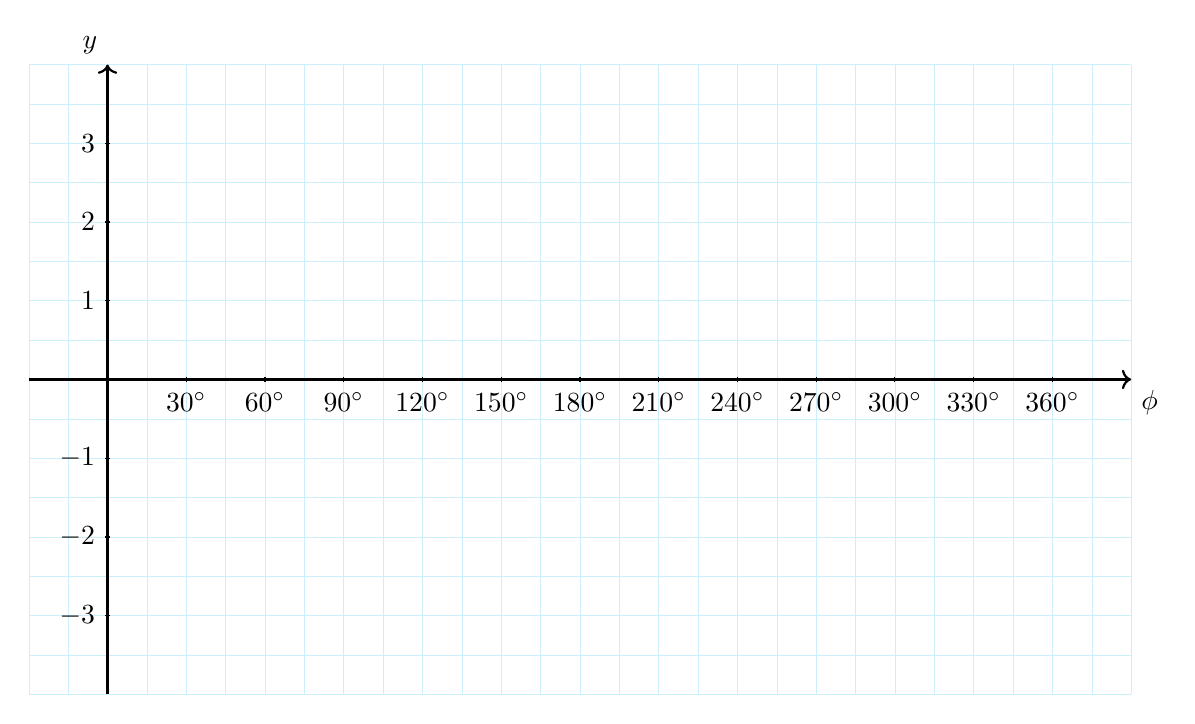
\begin{tikzpicture}
\draw[step = 0.5 cm, cyan!20 , very thin] (-1, -4) grid ( 13, 4);
\draw[thick, ->] (-1,0) -- (13,0) node[anchor = north west] {$\phi$};
\draw[thick, ->] (0,-4) -- (0,4) node[anchor = south east] {$y$};

\foreach \x [evaluate=\x as \degree using int(\x*30)] in {1,...,12}{ 
   \draw (\x cm, 1pt) -- (\x cm, -1pt) node[anchor = north] {$\degree^\circ$};
   }
\foreach \y in {-3,-2,-1,1,2,3}
   \draw (1pt, \y cm) -- (-1pt, \y cm) node[anchor = east] {$\y$};
\end{tikzpicture}}%% END Definition

\newcommand{\trigsysB}{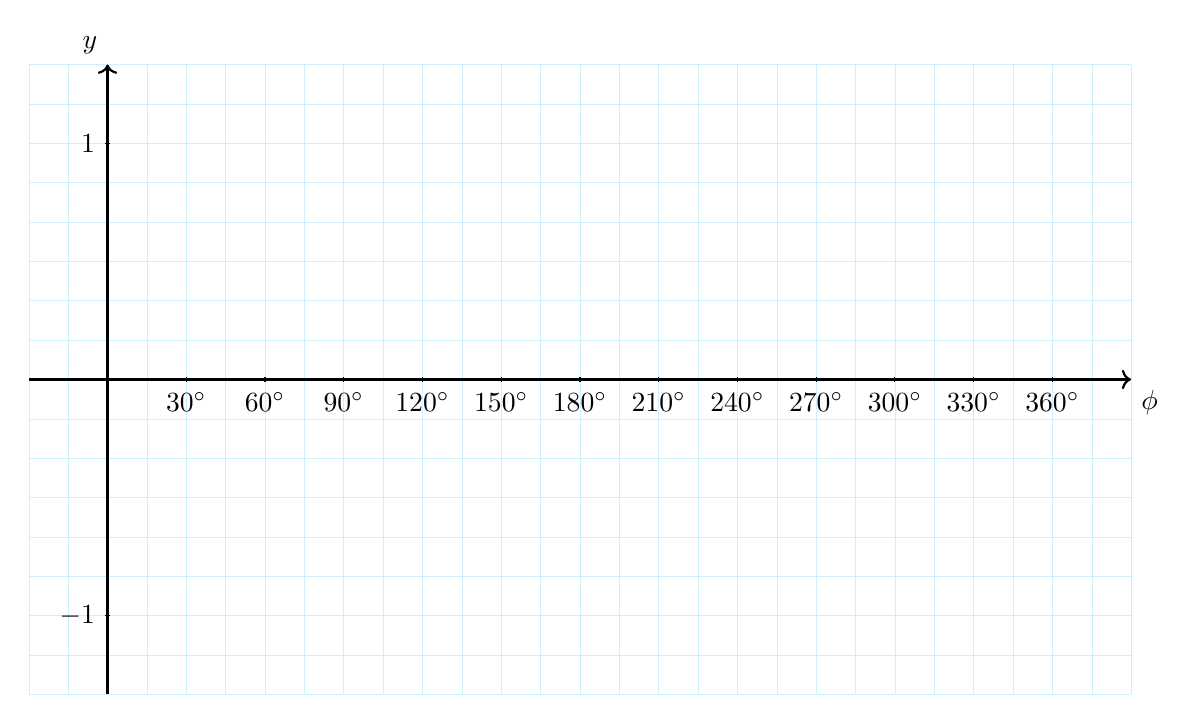
\begin{tikzpicture}\draw[step = 0.5 cm, cyan!20 , very thin] (-1, -4) grid ( 13, 4);
\draw[thick, ->] (-1,0) -- (13,0) node[anchor = north west] {$\phi$};
\draw[thick, ->] (0,-4) -- (0,4) node[anchor = south east] {$y$};

\foreach \x [evaluate=\x as \degree using int(\x*30)] in {1,...,12}{ 
   \draw (\x cm, 1pt) -- (\x cm, -1pt) node[anchor = north] {$\degree^\circ$};
   }
\foreach \y in {-1,1}
   \draw (1pt, \y *3cm) -- (-1pt, \y *3cm) node[anchor = east] {$\y$};

\end{tikzpicture}}%% END Definition

\newcommand{\trigsysC}{
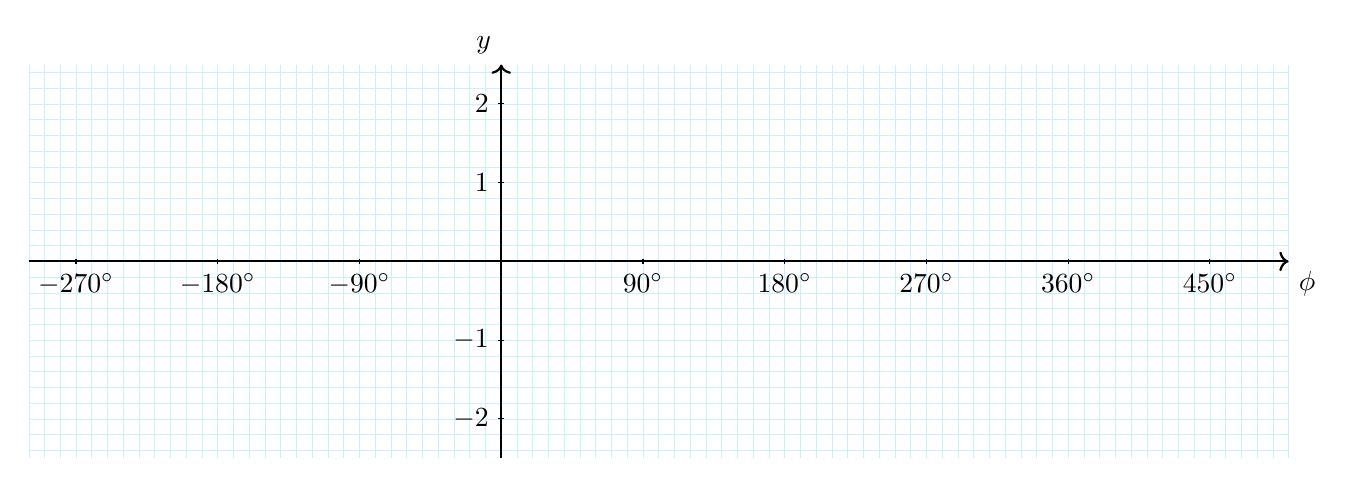
\begin{tikzpicture}
\draw[step = 0.2 cm, very thin, cyan!20] (-6, -2.5) grid ( 10, 2.5);
\draw[thick, ->] (-6,0) -- (10,0) node[anchor = north west] {$\phi$};
\draw[thick, ->] (0,-2.5) -- (0,2.5) node[anchor = south east] {$y$};

\foreach \x [evaluate=\x as \degree using int(\x*90)] in {-3,-2,-1,1,2,3,4,5}{ 
   \draw (\x *18mm, 1pt) -- (\x * 18mm, -1pt) node[anchor = north] {$\degree^\circ$};
   }
   
\foreach \y in {-2,-1,1,2}
   \draw (1pt, \y cm) -- (-1pt, \y cm) node[anchor = east] {$\y$};
\end{tikzpicture}}%% END Definition

\newcommand{\trigsysD}{
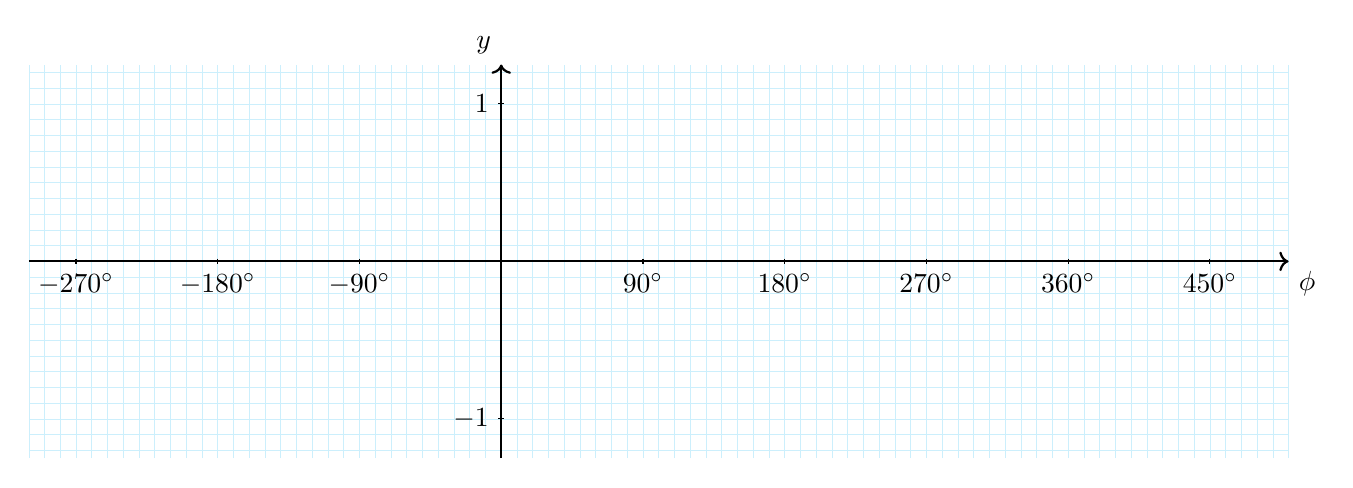
\begin{tikzpicture}
\draw[step = 0.2 cm, very thin, cyan!20] (-6, -2.5) grid ( 10, 2.5);
\draw[thick, ->] (-6,0) -- (10,0) node[anchor = north west] {$\phi$};
\draw[thick, ->] (0,-2.5) -- (0,2.5) node[anchor = south east] {$y$};

\foreach \x [evaluate=\x as \degree using int(\x*90)] in {-3,-2,-1,1,2,3,4,5}{ 
   \draw (\x *18mm, 1pt) -- (\x * 18mm, -1pt) node[anchor = north] {$\degree^\circ$};
   }
   
\foreach \y in {-1,1}
   \draw (1pt, \y *2cm) -- (-1pt, \y *2cm) node[anchor = east] {$\y$};
\end{tikzpicture}}%% END Definition


\newcommand{\trigsysDsin}{
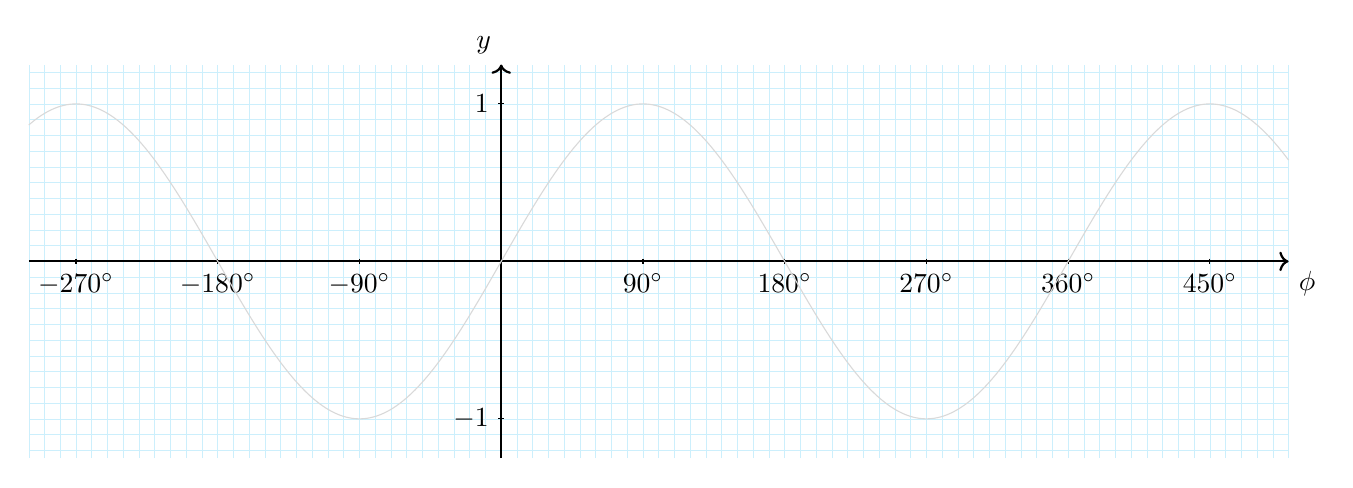
\begin{tikzpicture}
\draw[step = 0.2 cm, very thin, cyan!20] (-6, -2.5) grid ( 10, 2.5);
\draw[thick, ->] (-6,0) -- (10,0) node[anchor = north west] {$\phi$};
\draw[thick, ->] (0,-2.5) -- (0,2.5) node[anchor = south east] {$y$};

\foreach \x [evaluate=\x as \degree using int(\x*90)] in {-3,-2,-1,1,2,3,4,5}{ 
   \draw (\x *18mm, 1pt) -- (\x * 18mm, -1pt) node[anchor = north] {$\degree^\circ$};
   }
   
\foreach \y in {-1,1}
   \draw (1pt, \y *2cm) -- (-1pt, \y *2cm) node[anchor = east] {$\y$};

\draw[domain=-6:10,smooth,samples=200,variable=\x,gray!30] plot ({\x},{2*sin(\x*50)});
\end{tikzpicture}}%% END Definition

\newcommand{\trigsysDcos}{
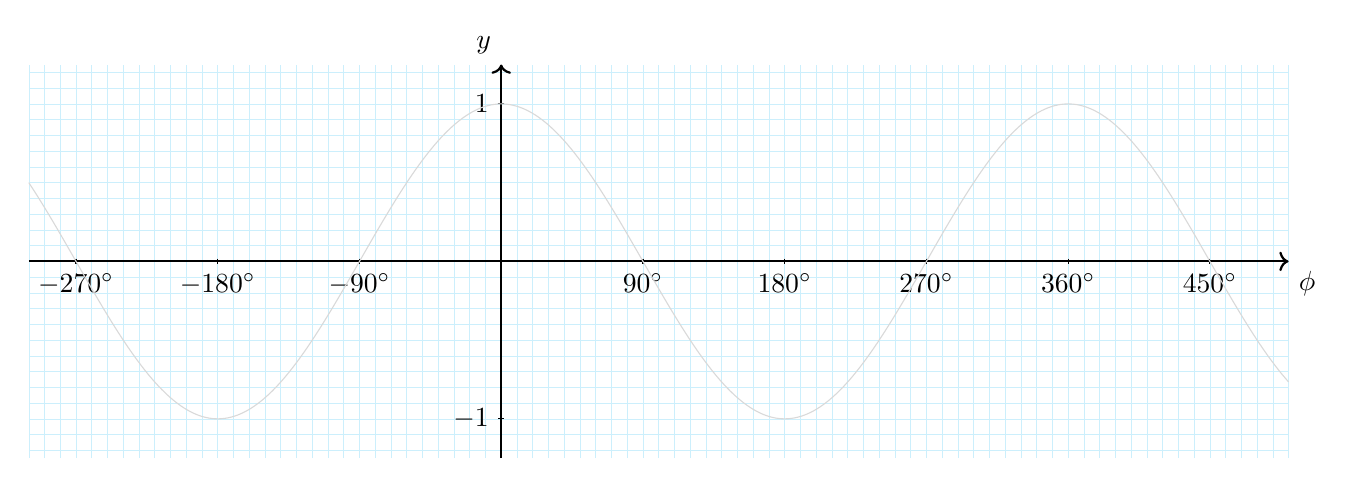
\begin{tikzpicture}
\draw[step = 0.2 cm, very thin, cyan!20] (-6, -2.5) grid ( 10, 2.5);
\draw[thick, ->] (-6,0) -- (10,0) node[anchor = north west] {$\phi$};
\draw[thick, ->] (0,-2.5) -- (0,2.5) node[anchor = south east] {$y$};

\foreach \x [evaluate=\x as \degree using int(\x*90)] in {-3,-2,-1,1,2,3,4,5}{ 
   \draw (\x *18mm, 1pt) -- (\x * 18mm, -1pt) node[anchor = north] {$\degree^\circ$};
   }
   
\foreach \y in {-1,1}
   \draw (1pt, \y *2cm) -- (-1pt, \y *2cm) node[anchor = east] {$\y$};

\draw[domain=-6:10,smooth,samples=200,variable=\x,gray!30] plot ({\x},{2*cos(\x*50)});
\end{tikzpicture}}%% END Definition


%%

\usepackage{bbwLayoutPageSty}


%%%%%%%%%%%%%%%  H E A D E R   &   F O O T E R %%%%%%%%%%%%%%%%%%%%
%% Headers
\fancyhf[HL]{\makebox{\includegraphics[width=30mm]{logos/bbw.pdf}}}%%
\fancyhf[HC]{\metaHeaderLine{}}%%
\fancyhf[FR]{\tiny{\shortAuthor{} (\today{})}}%%

\newcommand{\arbeitsblattHeader}{%%
  \begin{center}%%
    {\Large \fontfamily{qhv}\selectfont \arbeitsblattTitel{}}%%
\end{center}}%%


%%%%%%%%%%%%%%%%%%%%%%%%%%%%%%%%%%%%%%%%%%%%%%%%%%%%%%%%%%%%%%%%%%

\usepackage{amssymb} %% für \blacktriangleright
\renewcommand{\metaHeaderLine}{Skalarprodukt}
\renewcommand{\arbeitsblattTitel}{Vektorgeometrie in $\mathbb{R}^3$}

\begin{document}%%
\arbeitsblattHeader{}

\newcounter{aufgabennummer}
\setcounter{aufgabennummer}{1}


\newcommand\aufgabeML[2]{\begin{samepage}%%
\textbf{Aufgabe \arabic{aufgabennummer}:}\,\,\\
#1%%\\  \TRAINER{#2}
%%
\TRAINER{#2}%%abplz{5.2}
\noTRAINER{\mmPapierBisEndeSeite}
%%\end{samepage}
\stepcounter{aufgabennummer}%%
\end{samepage}%%
}%%


\section{Skalarprodukt}

 Es bezeichne jeweils $a = |\vec{a}|$.


\subsection{Formel zum Skalarprodukt}


\aufgabeML{ Gegeben sind die Vektoren $\vec{p}$ und $\vec{q}$ mit
$$p=37\hspace{11mm}q=42\hspace{1mm}\text{ und } \angle (\vec{p},\vec{q}) = 18\degre$$}%%
{Berechnen Sie das Skalarprodukt: $$\vec{p}\circ\vec{q} = \LoesungsRaum{37\cdot{}42\cdot\cos(18\degre)\approx 1477.9418}$$}


\aufgabeML{
Gegeben sind die Vektoren $\vec{r}$ und $\vec{s}$ mit: 
$$r=20\hspace{11mm}s=30\hspace{1mm}\text{ und } \angle
(\vec{r},\vec{s}) = 0\degre$$}{$$\vec{r}\circ\vec{s} = \LoesungsRaum{20\cdot{}30\cdot\cos(0\degre)=600}$$}


\aufgabeML{Berechnen Sie den Winkel zwischen $\vec{a}$ und $\vec{b}$.
$$\vec{a}\circ\vec{b}=18\hspace{11mm}a=9\hspace{11mm}b=8$$}{$$\angle(\vec{a},\vec{b})= \LoesungsRaum{=\arccos\left(\frac{\vec{a}\circ\vec{b}}{a\cdot{}b}\right)
  = \arccos{}\left(\frac{18}{9\cdot{}8}\right)\approx 75.52\degre}$$}

\aufgabeML{Berechnen Sie den Winkel zwischen $\vec{a}$ und $\vec{b}$.
$$\vec{a}\circ\vec{b}=56\hspace{11mm}a=7\hspace{11mm}b=8$$}{$$\angle(\vec{a},\vec{b})= \LoesungsRaum{=\arccos\left(\frac{\vec{a}\circ\vec{b}}{a\cdot{}b}\right)
  = \arccos{}\left(\frac{56}{7\cdot{}8}\right)\approx 0\degre}$$}



\aufgabeML{Berechnen Sie den Winkel zwischen $\vec{a}$ und $\vec{b}$.
$$\vec{a}\circ\vec{b}=0\hspace{11mm}a=1.41421\hspace{11mm}b=1.73205$$}{$$\angle(\vec{a},\vec{b})= \LoesungsRaum{=\arccos\left(\frac{\vec{a}\circ\vec{b}}{a\cdot{}b}\right)
  = \arccos{}\left(\frac{0}{a\cdot{}b}\right)\approx 90\degre}$$}

\aufgabeML{Berechnen Sie den Wert des Skalarproduktes, wenn bekannt
  isd, dass der Winkel zwischen den zwei Vektoren $\\vec{u}$ und
  $\vec{v}$ $45\degre$ beträgt und zusätzlich folgendes gilt:
 $$|\vec{u}|= 3 \text{ und } |\vec{v}|=4$$
}{...}


\aufgabeML{Seien $\vec{u}$ und $\vec{v}$ zwei Vektoren. Berechnen Sie
den Zwischenwinkel, wenn gilt:

a) $\vec{u}\circ{}\vec{v} = -u\cdot{}v$

b) $ \frac12ab = \vec{u}\circ{}\vec{v} $


}{...}

\aufgabeML{Zeigen Sie, mit der Definition des Skalarproduktes über den Cosinus, dass gilt:

$$\vec{u}\circ{}\vec{u} = u^2$$}{

Es gilt $$\vec{u}\circ{}\vec{v} = uv\cdot{}\cos(\gamma)$$ mit
$\gamma$  = Zwischenwinkel zwischen $\vec{u}$ und $\vec{v}$.

Wenn die Vektoren kollinear sind, so ist $\gamma=0$ und $\cos(\gamma)
= 1$

Somit ist

$$\vec{u}\circ{}\vec{u} = u\cdot{}u\cdot{}\cos(0\degre) = u\cdot{}u = u^2$$
}


\aufgabeML{%%
Gegeben sind die Vektoren $\vec{u} = \Spvek{2;0;-1}$, $\vec{v}
= \Spvek{1;-1;1}$ und $\vec{w} = \Spvek{0;1;-2}$.

Berechnen Sie mit dem Taschenrechner die folgende Summe:
$$(4\vec{u}\circ{}\vec{v}) + (\vec{u}\circ{}2\vec{w})
= \LoesungsRaum{8}$$
Tipp: \texttt{dotp} berechnet das Skalarprodukt auf dem tiNSpire.
}{%%
TR
}%% end AufgabeML





\aufgabeML{Für das Skalarproduk gilt das Distributivgesetz
folgendermaßen:

$$\vec{a}\circ{} (\vec{u} + \vec{v}) =  \vec{a}\circ{} \vec{u}
+ \vec{a}\circ{}\vec{v} $$
Berechnen Sie mit diesem Wissen den Winkel zwischen den Vektoren
$\vec{q}$ und $\vec{r}$, wenn folgendes gegeben ist:

$$q = 9 \text{, } r=2 \text{ und } \vec{r}\circ{}(\vec{q}-3\vec{r}) = 5$$
}{%% Lösungsteil
Es folgt:

$$\vec{r}\circ{}\vec{q} - 3\vec{r}\circ{}\vec{r} = 5$$

Wegen
$$\vec{r}\circ{}\vec{r} = r^2 = 4$$
gilt

$$\vec{r}\circ{}\vec{q} - 3\cdot{}4 = 5.$$

Daher:
$$\vec{r}\circ{}\vec{q} = 17 = rq\cdot{}\cos(\alpha)$$

Setzen wir unser $rq=2\cdot{}9=18$ ein, so erhalten wir:
$$17 = 18\cos{\alpha}$$

Nach $\alpha$ auflösen:
$$\alpha=\arccos\left(\frac{17}{18}\right) \approx 19.1881\degre$$

}

\subsection{Skalarprodukt aus gegebenen Vektoren berechnen}


\aufgabeML{Berechnen Sie $\vec{r}\circ\vec{s}$:
$$\vec{r} = \Spvek{6;-5} \hspace{11mm}\vec{s}=\Spvek{-6;-4}$$}%%
{$$\vec{r}\circ{}\vec{s} = \LoesungsRaum{-16}$$}

\aufgabeML{Berechnen Sie $\vec{r}\circ\vec{s}$:
$$\vec{r} = \Spvek{6;6;-3} \hspace{11mm} \vec{s}=\Spvek{-0.5;5;9}$$}%%
{$$\vec{r}\circ{}\vec{s} = \LoesungsRaum{0 \hspace{11mm}(=-3+30-27)}$$}
\TRAINER{\newpage}


\aufgabeML{%%
Bestimmen Sie das Skalarprodukt der Vektoren $\vec{u}$ und $\vec{v}$:
%% RoMi
$$\vec{u} = \Spvek{3;-4;6} \text{ und } \vec{v} = \Spvek{2;3;-1}$$
}{%%
}%% end AufgabeML



\aufgabeML{%%
Gegeben sind die Vektoren $\vec{a} = \Spvek{1;2}$,
$\vec{b}=\Spvek{-3;2}$, $\vec{c}=\Spvek{-4;-1}$ und $\vec{d}
= \Spvek{-1;3}$.

Berechnen Sie $(\vec{a} - 2\vec{c})\cdot{}(3\vec{b}-\vec{d})$
}{%%
 Lösung: $-60$
}%% end AufgabeML


\subsection{Parameter bestimmen, wenn Winkel gegeben}



\aufgabeML{Bestimmen Sie den Parameter $x$ von Hand so, dass die beiden
Vektoren $\vec{u}$ und $\vec{v}$ einen Winkel von 45 Grad
einschließen:
$$\vec{u} = \Spvek{1;1;0} \hspace{11mm} \vec{v}=\Spvek{2;1;x}$$}%%
{$$t = \LoesungsRaum{\pm 2}$$ }%% end aufgabeML
\TRAINER{..., denn $\cos{45\degre} = \frac{\sqrt2}2$ und dies ist
gleich $\frac{\vec{u}\circ\vec{v}}{uv} = \frac{1+2}{\sqrt{2}\cdot{}\sqrt{x^2+5}}$}



\aufgabeML{Bestimmen Sie den Parameter $s$ mit dem Taschenrechner so, dass die beiden
Vektoren $\vec{a}$ und $\vec{b}$ einen Winkel von 60 Grad
einschließen:
$$\vec{a} = \Spvek{2;3;4} \hspace{11mm} \vec{b}=\Spvek{5;s;8}$$}%%
{$$s = \LoesungsRaum{\frac{\sqrt{222691}-504}{7}\approx{}-4.5855}$$}
\TRAINER{Lösung mit TR: a und b definieren, dananach cos(60) =
dotp(a,b) / (norm(a) * norm(b)).}




\aufgabeML{%%
Berechnen Sie $x$ so, dass $\vec{a} = \Spvek{x;3;2}$ und $\vec{b}
= \Spvek{-4.5; 0; 1.5}$ einen Winkel von $62\degre$ einschließen.
}{%%
$x=-1.22$ (mit TR)
}%% end AufgabeML

\subsection{Winkel bestimmen}
\subsubsection{von Hand}

\aufgabeML{Bestimmen Sie von Handden Winkel zwischen Sie $\vec{u}$ und $ \vec{v}$:
$$\vec{u} = \Spvek{-1;3;5.5}\hspace{11mm}\vec{v}=\Spvek{2;-6;-11}$$}%%
{$$\angle(\vec{u},\vec{v}) = \LoesungsRaum{180\degre}$$
}%% end AufgabeML


\aufgabeML{Bestimmen Sie von Hand den Winkel zwischen Sie $\vec{u}$ und $ \vec{v}$:
$$\vec{u} = \Spvek{1;1;9} \hspace{11mm}\vec{v}= \Spvek{0.5;\frac12;4.5}$$}%%
{$$\angle(\vec{u},\vec{v}) = \LoesungsRaum{0\degre}$$}


\aufgabeML{Bestimmen Sie von Hand den Winkel zwischen Sie $\vec{u}$ und $ \vec{v}$:
$$\vec{u} = \Spvek{0;3;4} \hspace{11mm}\vec{v}= \Spvek{\sqrt{11};5;0}$$}%%
{$$\angle(\vec{u},\vec{v}) = \LoesungsRaum{60\degre}$$}

\aufgabeML{Bestimmen Sie von Hand den Winkel zwischen Sie $\vec{u}$ und $ \vec{v}$:
$$\vec{u} = \Spvek{-1;2;5} \hspace{11mm}\vec{v}= \Spvek{2;1;0}$$}%%
{$$\angle(\vec{u},\vec{v}) = \LoesungsRaum{90\degre}$$}

\subsubsection{mit Taschenrechner}

\aufgabeML{Bestimmen Sie den Winkel zwischen Sie $\vec{u}$ und $ \vec{v}$:
$$\vec{u} = \Spvek{-1;-2;-3} \hspace{11mm} \vec{v}=\Spvek{4;5;-6}$$}%%
{$$\angle(\vec{u},\vec{v}) = \LoesungsRaum{\arccos\left(\frac{2\cdot{}\sqrt{22}}{77}\right) \approx 83.00\degre}$$}


\aufgabeML{Bestimmen Sie den Winkel zwischen Sie $\vec{u}$ und $ \vec{v}$:
$$\vec{u} = \Spvek{-12;-7.5;-3.4} \hspace{11mm} \vec{v}=\Spvek{-4.5;2.4;3.8}$$}%%
{$$\angle(\vec{u},\vec{v}) = \LoesungsRaum{\arccos\left(\frac{2\cdot{}\sqrt{22}}{77}\right) \approx 75.6\degre}$$}

\subsection{Winkel zwischen Koordinatenachsen}



\aufgabeML{%%i
Welche drei Winkel bildet der Vektor $\vec{v}$ je mit den drei
Koordinatenachsen? Berechnen Sie von Hand!

$$\vec{v} = \Spvek{3\cdot{}\sqrt{3}; 0; 3}$$
}{%%
$x$-Achse: 30 Grad

$y$-Achse: 90 Grad

$z$-Achse: 60 Grad
}%% end AufgabeML



\aufgabeML{%%i
Ein Ortsvektor $\vec{r}$ mit Länge $v$ schließt mit der $x$- und der
$y$-Achse je einen Winkel von $\frac{\pi}3$ ein.

Bestimmen Sie von Hand den Winkel zwischen $\vec{r}$ und der $z$-Achse.


}{%%
Der Winkel misst $\frac{\pi}4$ (=$45\degre$ =$135\degre$, doch beim Winkel zwischen
zwei Geraden wird immer der kleinere genommen), egal, wie lang der Vektor ist.
}%% end AufgabeML


\subsubsection{Aufgaben mit Taschenrechner}



\aufgabeML{%%i
Welche Winkel bildet der Vektor $\vec{v}$ mit den drei
Koordinatenachsen?

$$\vec{v} = \Spvek{4;-11;1}$$
}{%%
Mit der $x$-Achse: 70.093 Grad

Mit der $y$-Achse: 20.547 Grad

Mit der $z$-Achse: 85.117 Grad
}%% end AufgabeML

\aufgabeML{%%i
Welche Winkel bildet der Vektor $\vec{v}$ mit den drei
Koordinatenachsen?

$$\vec{v} = \Spvek{6.5; 5.5; 4}$$
}{%%
Mit der $x$-Achse: 46.3 Grad

Mit der $y$-Achse: 54.2 Grad

Mit der $z$-Achse: 64.8 Grad
}%% end AufgabeML


\aufgabeML{%%i
Ein Ortsvektor bildet mit der $x$-Achse einen Winkel von $38\degre$
und mit der $y$-Achse einen von $117\degre$. Berechnen Sie den Winkel
mit der $z$-Achse.
}{%%
$\alpha_z = 65.427\degre$
}%% end AufgabeML



\aufgabeML{Berechnen Sie den Winkel $\alpha$ zwischen der $xy$-Ebene und dem
Vektor $\vec{q}$:

$\vec{q}=\Spvek{-3;6;2}$}%%
{$$\alpha=\LoesungsRaum{\arccos(\frac{\vec{q}\circ{}\vec{p}}{qp})\text{
mit p = Projektion auf xy-Ebene (-3;6;0)} \approx 16.6015\degre}$$
}


\subsection{Orthogonale Vektoren}
(Skalarprodukt = 0)
\subsubsection{Aufgaben von Hand}

\aufgabeML{
Gegeben sind Vektoren $\vec{a}$ und $\vec{b}$ mit
$$a=11.3\hspace{11mm}b=17.853\hspace{1mm}\text{ und } \angle
(\vec{a},\vec{b}) = 90\degre$$}{$$\vec{a}\circ\vec{b} = \LoesungsRaum{11.3\cdot{}17.853\cdot\cos(90\degre)=0}$$}

\aufgabeML{Bestimmen Sie den Parameter $t$ von Hand so, dass die beiden
Vektoren $\vec{p}$ und $\vec{q}$ einen Winkel von $\frac{\pi}2$
einschließen:
$$\vec{p} = \Spvek{1;t;2} \hspace{11mm} \vec{q}=\Spvek{3;1;t}$$}%%
{$$t = \LoesungsRaum{-1}$$ }%% end aufgabeML
\TRAINER{..., denn bei 90 Grad ist das Skalarprodukt = 0 und somit
muss $3t+3 = 0$ sein. Dies geht nur, wenn $t=-1$}



\aufgabeML{%%i
Bestimmen Sie sämtliche WVektoren, die senkrecht zum Vektor $\vec{v}$
stehen und die selbe Länge wie $\vec{v}$ haben:

$$\vec{v} = \Spvek{-3; 1}$$
}{%%
$\Spvek{1;3}$ und $\Spvek{-1;-3}$
}%% end AufgabeML

\aufgabeML{%%i
Bestimmen Sie den Parameter $n$, sodass die beiden folgenden Vektoren
senkrecht zueinaned stehen:

$$\Spvek{n;1;-3} \hspace{11mm}  \Spvek{4;-2;n}$$
}{%%
$n=2$
}%% end AufgabeML


\aufgabeML{%%i
Bestimmen Sie den Parameter $p$ so, adass die beiden Vektoren
senkrecht aufeinander stehen:

$$\vec{u} = \Spvek{p;2;3} \hspace{33mm}  \vec{v} = \Spvek{1;0;-2}$$
}{%%
$p=6$
}%% end AufgabeML


\aufgabeML{%%i
Bestimmen Sie den Parameter $p$ so, adass die beiden Vektoren
senkrecht aufeinander stehen:

$$\vec{u} = \Spvek{2p;2;-4} \hspace{33mm}  \vec{v} = \Spvek{p;-8;p}$$

(Tipp beim Lösen der quadratischen Gleichung: Zweiklammeransatz)
}{%%
$p_1=-2, p_2=4$
}%% end AufgabeML



\aufgabeML{%%i
Bestimmen Sie $x$ und $z$ so, dass der Vektor $\vec{r}=Spvek{x;3;z}$
senkrecht auf den beiden Vektoren steht:

$$\vec{u} = \Spvek{5;4;9} \hspace{33mm}  \vec{v} = \Spvek{2;5;-1.5}$$

(Tipp beim Lösen der quadratischen Gleichung: Zweiklammeransatz)
}{%%
$x=-6, z=2$
}%% end AufgabeML

\aufgabeML{%%i
Bestimmen Sie den Parameter $y$ so, dass das Dreieck $\triangle ABC$
bei $\beta (= \angle ABC)$ rechtwinklig wird:

$$A=(2|1|3); B=(4|y|1) \text{ und } C=(2|4|0)$$
}{%%
Lösungen: $y=2$ oder $y=3$

Weg:

$\vec{a} = \overrightarrow{BC}=\Spvek{-2;4-y;-1}$

$\vec{b} =\overrightarrow{AB} = \Spvek{2;y-1;-2}$

Skalarprodukt über die Komponenten bestimmen und = 0 setzen.
}%% end AufgabeML



\subsubsection{Aufgaben mit Taschenrechner}
\aufgabeML{%%i
Bestimmen Sie sämntliche Vektoren der Länge 6, die senkrecht zu
$\vec{u}$ und zu $\vec{v}$ stehen:

$$\vec{u} = \Spvek{2;1;-2}\hspace{11mm} \vec{v} = \Spvek{-1;0;4}$$
}{%%
Lösung: $\pm \Spvek{3.3; -4.94; 0.82}$
}%% end AufgabeML


\aufgabeML{%%i
Berechnen Sie $k$ so, dass $\vec{u}$ und $\vec{v}$ einen Winkel von
$90\degre$ einschließen:

$$\vec{u} = \Spvek{-1;k+2;3} \hspace{11mm} \vec{v} = \Spvek{2; k-3; k}$$
}{%%
$L_k = \{-4; 2\}$
}%% end AufgabeML







































\aufgabeML{%%i

}{%%

}%% end AufgabeML

\aufgabeML{%%i

}{%%

}%% end AufgabeML

\aufgabeML{%%i

}{%%

}%% end AufgabeML

\aufgabeML{%%i

}{%%

}%% end AufgabeML

\aufgabeML{%%i

}{%%

}%% end AufgabeML




\end{document}
